\chapter{IMPLEMENTATION} 
\label{sec.implementation}
Based on the design introduced in \S{\ref{sec.design}}, we implement a 
secure network testbed. We describe the implementation details of our system 
in this section. It is important to acknowledge that the \sysname benefits from the design and implementation of Seattle Testbed, an open experimental platform for researchers and educators to understand the real world network. Over the past six years, the Seattle Testbed has been used in a variety of different experiments and its use is spread across the world. A core design principle of this testbed is the implementation of Repy sandbox on user devices. The sandbox has several goals. First of all, it must be able to run experiment code while representing as little risk to user's security as possible. For instance, programs are only allowed to operate inside of a sandbox, ensuring user's sensitive information on host are kept safe and private. In addition, sandbox must provide performance isolation for experiment code to prevent them from consuming too much CPU, memory, disk I/O and network bandwidth. The basic design of the Repy for OpenWrt described below was leveraged from the Seattle design.

\section{Core Components}
\subsection{Sandbox}
\label{sec.sandbox}
The core sandbox - \sandboxname, which is extended from Repy (Restricted Python), a Python-based programming language sandbox that minimizes the risk of bugs by providing security isolation and performance isolation. Experimenters in \sysname use this Python-like programming interface to write experiment code. Currently. Repy provides programmers with the ability to read and write files on the disk, send TCP and UDP traffic and some utility methods to retrieve time etc. In order to run broadband and wireless network experimentation on home wireless routers, \sysname extends the Repy and adds the capabilities to access linux kernel API and active measurement tools (e.g., Ping, Traceroute). The programming interface exposed to the repy-scripts has been extended to include methods to list available access points and connected clients, receive network traffic data from \texttt{/proc} file system and do common active measurements (Ping and Traceroute). To avoid resource limitation, we define a non-renewable and fungible resource\cite{li2015fence} (\texttt{procfs}) to control the resource of reading \texttt{/proc} file system. 

Another important feature of \sandboxname allows us to define a policy for its programming interface. For example, the sandbox can anonymize the MAC address of available access points and blacklist home user's LAN. The policy enforcement is presented in \S{\ref{sec.policy}}. We focus on the security and performance isolation of \sandboxname in this section.
\begin{itemize}
\item \textbf{Performance isolation: }Each router running \sysname uses an uniform resource control method to allocate a fixed percentage (usually 50\%) of the router's CPU, memory, brandwidth, disk and other resources to one or more sandboxes. To achieve this, Repy uses operating system hooks to monitor the amount of CPU and memory available to an experiment. To restrict other resources such as network bandwidth and disk I/O, Repy checks those calls that access these resources, and preventing or delaying the execution of these calls if they exceed configured quota. When sandbox is started, it reads a configure file that lists the resources allocated to the experiment. Each line contains a resource type and quantity. For example, \texttt{resource diskused 100000000} means that 100 million bytes disk memory can be used at most. Due to this isolation, sandbox does not allow experiment to consume a lot of resources and ensure experiment not affect Internet connectivity.

\item \textbf{Security isolation: }Repy sandbox has a small, self-contained kernel as its trusted computing base (TCB). In order to minimize the risk of bugs, the TCB is small (only include classic Python classes) so that it is less likely to have security risks than other complex kernels. This sandbox also uses \textit{security layers} to push library functionality out of the sandbox kernel, therefore it is helpful to mitigate security risks in libraries. 

\end{itemize}
\subsection{Package Builder}
\label{sec.packagebuilder}
Any experimenter can easily obtain a customized installer for \sysname which provides access to sandboxes in any way. The goal of package builder is make it incredibly easy to post our platform to OpenWrt. Currently we use OpenWrt SDK to build installer. These can be given out by an experimenter who does not want use a clearinghouse. In addition, these installers can be bundled with other components to allow the experimenter direct control over safe experimental sandboxes on their end user devices.

\subsection{Node Manager}
\label{sec.nodemanager}
Node manager\cite{nodemanager} ensures that sandboxes are correctly assigned to experimenters and experimenters can control those sandboxes safely. The Node manager is based on prior work on Seattle Testbed, but is customized to the OpenWrt. For example, \sysname runs on a home wireless router as background process. Starting it at booting time of the router is implemented by an init.d script instead of crontab. Cryptographically signed messages is used to perform authentication of remote experimenters who are identified by their public keys. An experimenter can perform actions on the sandbox such as starting and stoping an experiment, uploading code, collecting files and data. The node manager is running in a sandbox to check whether the interface is accessed. The node manager also includes code to traverse NAT gateways and firewalls so that it is contactable even if the router does not have a public IP address. 

\subsection{Software Updater}
\label{sec.softwareupdater}
Software updater allows SOAR-enabled router to search for and update new release automatically. It runs in background, sleeps some random amount of time (30min - 1hour) to check with the package builder if there exists a new update. It then downloads the new installer from package builder and replaces the old installer. 

\subsection{Lookup Service}
\label{sec.lookupservice}
A lookup service allows experimenter to locate the corresponding sandboxes. We currently use OpenDHT\cite{rhea2005opendht} as a distributed way to store data. Each sandbox advertise their availability via OpenDHT using a public key. OpenDHT runs on a variety of PlanetLab nodes and replicates data.

\subsection{Experiment Manager}
\label{sec.seash}
An experiment manager provides experimenters with a simple interface for interacting with the resource manager on remote devices. The primary interactive service manager used in \sysname is \textit{seash}\cite{seash}. It provides an interactive shell to the experimenters. \textit{seash} exchanges cryptographically signed communication with sandboxes to control experiments and upload files. Also, the experiment manager supports contacting routers which in networks behind NAT gateways and firewalls to satisfy the reality of today's network.

\section{Sandbox Extensions}
\label{sec.extensions}
Extensions enhance the functionality of the Repy sandbox and allow a wide range of network measurements on home wireless router. First, we implemented system hooks call \textit{openwrt module} to interact with a variety of wired and wireless network information through Linux kernel API. Currently, implemented \textit{openwrt module} is supported to learn about configured network interfaces statistics, connected devices, nearby WiFi access points and channel utilization. While \textit{openwrt module} is the system hooks with read access to valuable data, they can not modify data. Additionally, we also implemented a \textit{general modules} to provide two active measurement tools (Ping and Traceroute). We choose a pure raw socket method to implement them so that they will be supported across a variety of operating systems. 

\textbf{Protecting command injection.} Command injection is an attack which execute arbitrary commands on the host operating system by a vulnerable application. The possible reason of command injection attacks is insufficient input validation. \sysname sanitizes the call arguments, handles onerous output parsing, and returns results to the caller. One example is \texttt{scan} implementation. This function will run a system command \texttt{iw dev interface\_name station dump}. We will check whether interface name is legal, any illegal arguments will pose a security risk, such as \texttt{;ls} is able to show files in current directory. \sysname API never allows invocation of arbitrary system calls.

\begin{figure}%[h]
\centering
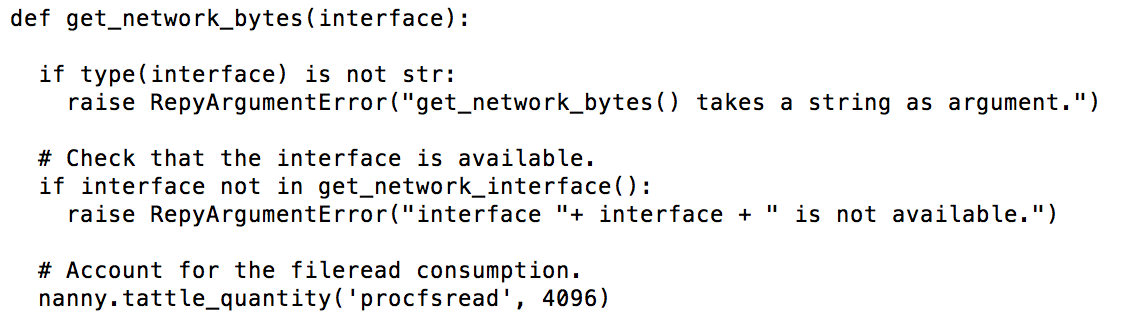
\includegraphics[width=0.8\columnwidth]{figure/nanny.png}
\caption{Additional codes in \sysname sandbox's \texttt{get\_network\_bytes()} call to make sure resource control and command injection protection.}
\label{fig-nanny}
\end{figure}

\textbf{Resource control.} Resource control is an important security mechanism. It provides protection from accidental or deliberate over-usage of resources by APIs affecting the service level of end host. Each new functions in SOAR-Repy define a resource type to record the amount of resource they consume. The specific function made depends on the type of resource being consumed. Figure \ref{fig-nanny} shows some of codes in \texttt{get\_network\_bytes()}. First of all, we check whether the argument is legal and available. The \texttt{tattle\_quantity()} call charges for the consumed fileread. When a \sysname starts, it reads a text file that lists the resources allocated to the platform. Each line contains a resource type and quantity. For example, \texttt{resource procfsread 100000} sets the allowed consumption of reading \texttt{/proc} filesystem to 100 thousand bytes. When experiment codes try to exceed the limit, it will be forcefully killed.

\section{Sandbox Policies}
\label{sec.policy}
In order for router owner to participate safely in \sysname, he should have the ability to decide policies on his own. For instance, he should know the amount of resources \sysname will use on his router and the capabilities experiment code can access to. We have mentioned the resource control in \S{\ref{sec.sandbox}}. To restrict capabilities, the sandbox in \sysname provides a flexible policy enforcement method that uses Repy's security layer to help router owner to decide policies. Sandbox can interject code to control the behaviour of these calls through a system call interposition technique. Using this technology, a sandbox policy can (1) restrict capability access, such as blocking sending TCP or UDP packet to protect LAN, and (2) reduce precision of returned data from a router, such as returning the number of connected devices rather than detailed information of each connected device.

\subsection{Reducing Data Precision}
Our sandbox may provides potentially inappropriate functions such as network traffic capture that disclose the home network behaviour pattern of router owner. This kind of policies are able to change the behaviour of a function such as it can disable the returned value and the precision of a specified value returned. For instance, security layer could truncate access point MAC address to the manufacturer ID.

\begin{figure}%[h]
\centering
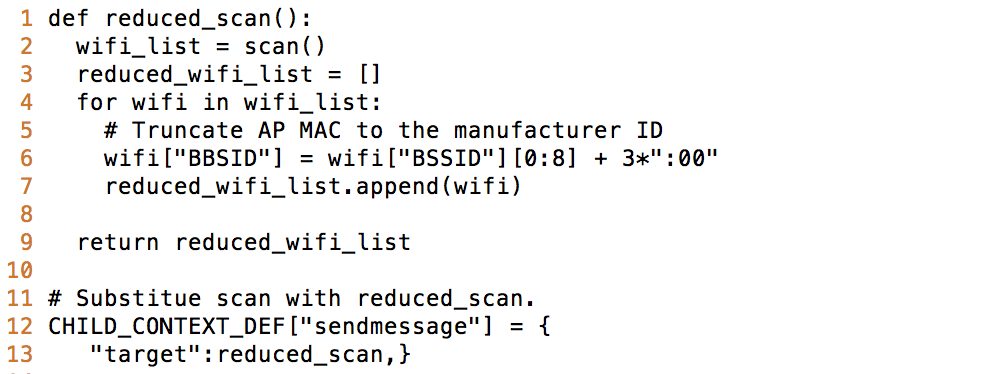
\includegraphics[width=0.8\columnwidth]{figure/example.png}
\caption{Using security layer to define a simple sandbox policy: truncate access point MAC address to the manufacturer ID.}
\label{fig-examplecode}
\end{figure}

As shown in figure~\ref{fig-examplecode}, whenever experiment code calls \texttt{scan()}, the security layer above replaces it with \texttt{reduced\_scan()}. Therefore, security layer is able to ensure router owner's policy.

\subsection{Restricting Capability Access}
This kind of policy is able to allow experimenters to restrict the code on home wireless router. For example, the experimenter may wants to restrict part of functionalities to satisfy router owner's need. It is also useful to save time to vet experiment code because most harmful capabilities are restricted. As a result, \sysname is able to maintain containment of experiment code despite bugs in libraries.
 